\documentclass[12pt,letterpaper]{article}
\usepackage[margin=0.65in,top=0.77in,bottom=0.65in,headheight=16pt,headsep=14pt,footskip=22pt]{geometry}
\usepackage[T1]{fontenc}
\usepackage{helvet}
\renewcommand\familydefault{\sfdefault}
\usepackage{tikz}
\usepackage{fancyhdr}
\usepackage{array}
\usepackage{xcolor}
\usepackage{microtype}
\usetikzlibrary{arrows.meta}
\definecolor{linkgrey}{gray}{0.48}
\definecolor{ink}{gray}{0.08}
\tikzset{available/.style={draw=linkgrey,line width=0.65pt},bought/.style={draw=ink,line width=2.4pt},place/.style={circle,draw=ink,line width=0.9pt,fill=white,inner sep=0pt},price/.style={fill=white,inner sep=1.4pt}}
\newcommand\pricedots[1]{\begin{tikzpicture}[baseline=-0.7ex]\foreach \i in {1,...,#1}{\fill (\i*0.135,0) circle (0.034);}\end{tikzpicture}}
\newcommand\coins[1]{\begin{tikzpicture}[baseline=-0.7ex]\foreach \i in {1,...,#1}{\draw[line width=0.6pt] (\i*0.21,0) circle (0.082);}\end{tikzpicture}}
\newcommand\Band{Grades K--5}
\pagestyle{fancy}\fancyhf{}
\fancyhead[L]{\small Week 53 / Connecting networks / \Band}
\fancyfoot[L]{\scriptsize Bellingham Math Circle / Week 53 / W53-networks-v2}
\fancyfoot[R]{\scriptsize\thepage}
\renewcommand\headrulewidth{0pt}\renewcommand\footrulewidth{0pt}
\setlength\parindent{0pt}\setlength\parskip{8pt}
\newcommand\problem[2]{\textbf{Problem #1:} #2\par}
\newcommand\cost{Cost: \rule{1.2cm}{0.4pt}}
\newcommand\writing[1]{\vspace{#1}\par}
\newcommand\swaprows{\begin{tabular}{@{}p{1.6cm}p{1.6cm}p{2.5cm}@{}}Return & Buy & New cost\\[3pt]\hline\\[10pt]\hline\\[10pt]\hline\\[10pt]\hline\\[10pt]\hline\end{tabular}}
% The diagram macros (\TriangleOne, ...) are defined at the start of the body by
% problems/00-diagram-macros.md, drawn by editable/student/diagrams.py from networks.json.
\begin{document}
\newcommand{\ExampleAvailable}{%
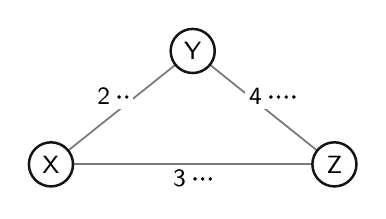
\begin{tikzpicture}[x=0.72cm,y=0.72cm,baseline=(current bounding box.center)]
\coordinate (X) at (0,0);
\coordinate (Y) at (2.5,2);
\coordinate (Z) at (5,0);
\draw[available] (X) -- (Y);
\draw[available] (Y) -- (Z);
\draw[available] (X) -- (Z);
\node[price,font=\small] at (1.09383,1.19522) {2\;\pricedots{2}};
\node[price,font=\small] at (3.90617,1.19522) {4\;\pricedots{4}};
\node[price,font=\small] at (2.50000,-0.25000) {3\;\pricedots{3}};
\node[place,minimum size=0.56cm,font=\small] at (X) {X};
\node[place,minimum size=0.56cm,font=\small] at (Y) {Y};
\node[place,minimum size=0.56cm,font=\small] at (Z) {Z};
\end{tikzpicture}
}

\newcommand{\ExamplePaid}{%
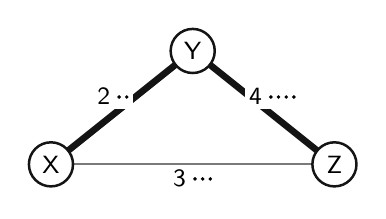
\begin{tikzpicture}[x=0.72cm,y=0.72cm,baseline=(current bounding box.center)]
\coordinate (X) at (0,0);
\coordinate (Y) at (2.5,2);
\coordinate (Z) at (5,0);
\draw[available] (X) -- (Y);
\draw[available] (Y) -- (Z);
\draw[available] (X) -- (Z);
\draw[bought] (X) -- (Y);
\draw[bought] (Y) -- (Z);
\node[price,font=\small] at (1.09383,1.19522) {2\;\pricedots{2}};
\node[price,font=\small] at (3.90617,1.19522) {4\;\pricedots{4}};
\node[price,font=\small] at (2.50000,-0.25000) {3\;\pricedots{3}};
\node[place,minimum size=0.56cm,font=\small] at (X) {X};
\node[place,minimum size=0.56cm,font=\small] at (Y) {Y};
\node[place,minimum size=0.56cm,font=\small] at (Z) {Z};
\end{tikzpicture}
}

\newcommand{\ExampleRecord}{%
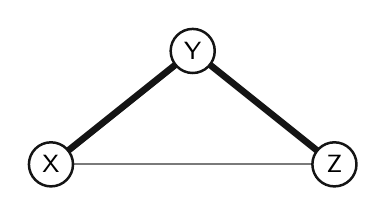
\begin{tikzpicture}[x=0.72cm,y=0.72cm,baseline=(current bounding box.center)]
\coordinate (X) at (0,0);
\coordinate (Y) at (2.5,2);
\coordinate (Z) at (5,0);
\draw[available] (X) -- (Y);
\draw[available] (Y) -- (Z);
\draw[available] (X) -- (Z);
\draw[bought] (X) -- (Y);
\draw[bought] (Y) -- (Z);
\node[place,minimum size=0.56cm,font=\small] at (X) {X};
\node[place,minimum size=0.56cm,font=\small] at (Y) {Y};
\node[place,minimum size=0.56cm,font=\small] at (Z) {Z};
\end{tikzpicture}
}

\newcommand{\TriangleOne}{%
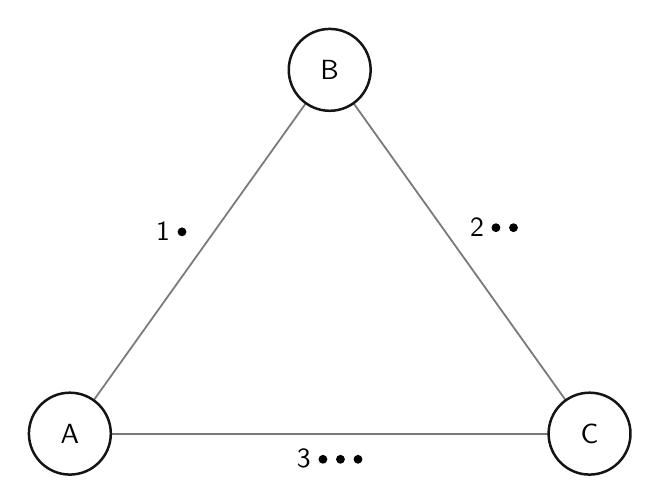
\begin{tikzpicture}[x=1.65cm,y=1.65cm,baseline=(current bounding box.center)]
\coordinate (A) at (0,0);
\coordinate (B) at (2,2.8);
\coordinate (C) at (4,0);
\draw[available] (A) -- (B);
\draw[available] (B) -- (C);
\draw[available] (A) -- (C);
\node[price,font=\normalsize] at (0.78042,1.55684) {1\;\pricedots{1}};
\node[price,font=\normalsize] at (3.26431,1.58879) {2\;\pricedots{2}};
\node[price,font=\normalsize] at (2.00000,-0.19394) {3\;\pricedots{3}};
\node[place,minimum size=1.04cm,font=\normalsize] at (A) {A};
\node[place,minimum size=1.04cm,font=\normalsize] at (B) {B};
\node[place,minimum size=1.04cm,font=\normalsize] at (C) {C};
\end{tikzpicture}
}

\newcommand{\TriangleTwo}{%
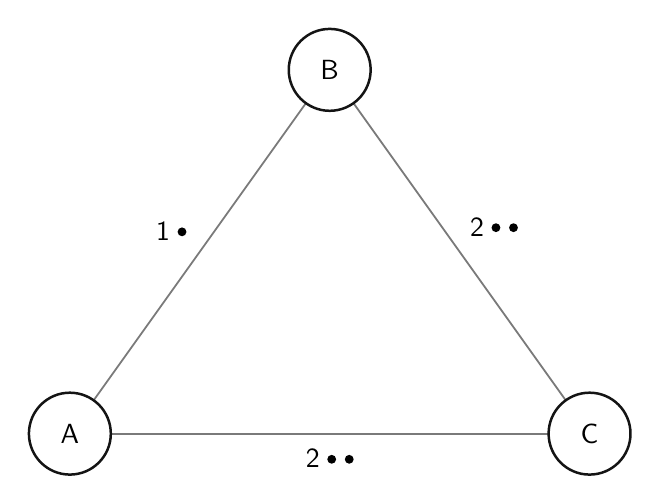
\begin{tikzpicture}[x=1.65cm,y=1.65cm,baseline=(current bounding box.center)]
\coordinate (A) at (0,0);
\coordinate (B) at (2,2.8);
\coordinate (C) at (4,0);
\draw[available] (A) -- (B);
\draw[available] (B) -- (C);
\draw[available] (A) -- (C);
\node[price,font=\normalsize] at (0.78042,1.55684) {1\;\pricedots{1}};
\node[price,font=\normalsize] at (3.26431,1.58879) {2\;\pricedots{2}};
\node[price,font=\normalsize] at (2.00000,-0.19394) {2\;\pricedots{2}};
\node[place,minimum size=1.04cm,font=\normalsize] at (A) {A};
\node[place,minimum size=1.04cm,font=\normalsize] at (B) {B};
\node[place,minimum size=1.04cm,font=\normalsize] at (C) {C};
\end{tikzpicture}
}

\newcommand{\FourTies}{%
\begin{tikzpicture}[x=2.25cm,y=2.25cm,baseline=(current bounding box.center)]
\coordinate (A) at (0,3);
\coordinate (B) at (0,0);
\coordinate (C) at (3.2,1.5);
\coordinate (D) at (6.4,1.5);
\draw[available] (A) -- (B);
\draw[available] (B) -- (C);
\draw[available] (A) -- (C);
\draw[available] (C) -- (D);
\draw[available] (A) -- (D);
\node[price,font=\normalsize] at (-0.17882,1.50000) {1\;\pricedots{1}};
\node[price,font=\normalsize] at (1.52289,0.91450) {1\;\pricedots{1}};
\node[price,font=\normalsize] at (1.52289,2.08550) {1\;\pricedots{1}};
\node[price,font=\normalsize] at (4.80000,1.64222) {2\;\pricedots{2}};
\node[price,font=\normalsize] at (3.24385,2.43710) {3\;\pricedots{3}};
\node[place,minimum size=1.04cm,font=\normalsize] at (A) {A};
\node[place,minimum size=1.04cm,font=\normalsize] at (B) {B};
\node[place,minimum size=1.04cm,font=\normalsize] at (C) {C};
\node[place,minimum size=1.04cm,font=\normalsize] at (D) {D};
\end{tikzpicture}
}

\newcommand{\FourTiesRecord}{%
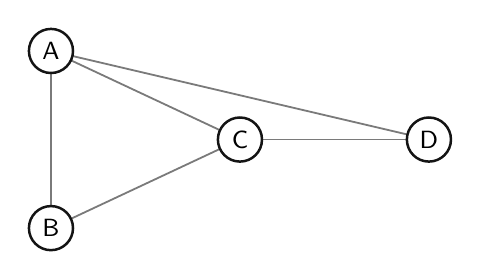
\begin{tikzpicture}[x=0.75cm,y=0.75cm,baseline=(current bounding box.center)]
\coordinate (A) at (0,3);
\coordinate (B) at (0,0);
\coordinate (C) at (3.2,1.5);
\coordinate (D) at (6.4,1.5);
\draw[available] (A) -- (B);
\draw[available] (B) -- (C);
\draw[available] (A) -- (C);
\draw[available] (C) -- (D);
\draw[available] (A) -- (D);
\node[place,minimum size=0.56cm,font=\small] at (A) {A};
\node[place,minimum size=0.56cm,font=\small] at (B) {B};
\node[place,minimum size=0.56cm,font=\small] at (C) {C};
\node[place,minimum size=0.56cm,font=\small] at (D) {D};
\end{tikzpicture}
}

\newcommand{\FourTrap}{%
\begin{tikzpicture}[x=2.25cm,y=2.25cm,baseline=(current bounding box.center)]
\coordinate (A) at (0,3);
\coordinate (B) at (0,0);
\coordinate (C) at (3.2,1.5);
\coordinate (D) at (6.4,1.5);
\draw[available] (A) -- (B);
\draw[available] (B) -- (C);
\draw[available] (A) -- (C);
\draw[available] (C) -- (D);
\draw[available] (A) -- (D);
\node[price,font=\normalsize] at (-0.17882,1.50000) {1\;\pricedots{1}};
\node[price,font=\normalsize] at (1.51072,0.94046) {2\;\pricedots{2}};
\node[price,font=\normalsize] at (1.49855,2.03358) {3\;\pricedots{3}};
\node[price,font=\normalsize] at (4.80000,1.64222) {4\;\pricedots{4}};
\node[price,font=\normalsize] at (3.25089,2.46712) {5\;\pricedots{5}};
\node[place,minimum size=1.04cm,font=\normalsize] at (A) {A};
\node[place,minimum size=1.04cm,font=\normalsize] at (B) {B};
\node[place,minimum size=1.04cm,font=\normalsize] at (C) {C};
\node[place,minimum size=1.04cm,font=\normalsize] at (D) {D};
\end{tikzpicture}
}

\newcommand{\FourTrapRecord}{%
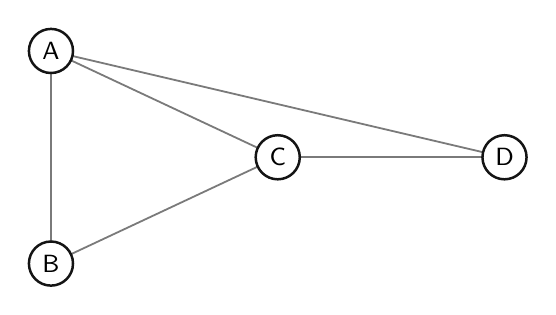
\begin{tikzpicture}[x=0.9cm,y=0.9cm,baseline=(current bounding box.center)]
\coordinate (A) at (0,3);
\coordinate (B) at (0,0);
\coordinate (C) at (3.2,1.5);
\coordinate (D) at (6.4,1.5);
\draw[available] (A) -- (B);
\draw[available] (B) -- (C);
\draw[available] (A) -- (C);
\draw[available] (C) -- (D);
\draw[available] (A) -- (D);
\node[place,minimum size=0.56cm,font=\small] at (A) {A};
\node[place,minimum size=0.56cm,font=\small] at (B) {B};
\node[place,minimum size=0.56cm,font=\small] at (C) {C};
\node[place,minimum size=0.56cm,font=\small] at (D) {D};
\end{tikzpicture}
}

\newcommand{\FiveTies}{%
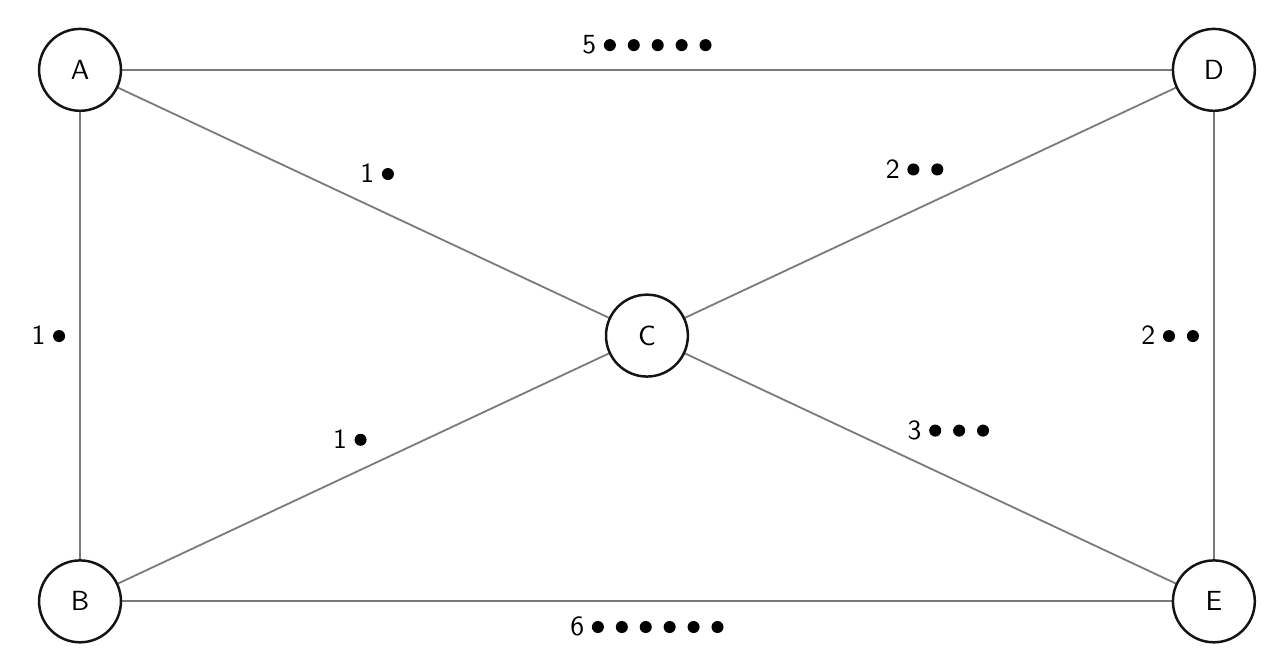
\begin{tikzpicture}[x=2.25cm,y=2.25cm,baseline=(current bounding box.center)]
\coordinate (A) at (0,3);
\coordinate (B) at (0,0);
\coordinate (C) at (3.2,1.5);
\coordinate (D) at (6.4,3);
\coordinate (E) at (6.4,0);
\draw[available] (A) -- (B);
\draw[available] (B) -- (C);
\draw[available] (A) -- (C);
\draw[available] (C) -- (D);
\draw[available] (D) -- (E);
\draw[available] (C) -- (E);
\draw[available] (A) -- (D);
\draw[available] (B) -- (E);
\node[price,font=\normalsize] at (-0.17882,1.50000) {1\;\pricedots{1}};
\node[price,font=\normalsize] at (1.52289,0.91450) {1\;\pricedots{1}};
\node[price,font=\normalsize] at (1.67711,2.41450) {1\;\pricedots{1}};
\node[price,font=\normalsize] at (4.71072,2.44046) {2\;\pricedots{2}};
\node[price,font=\normalsize] at (6.15364,1.50000) {2\;\pricedots{2}};
\node[price,font=\normalsize] at (4.90145,0.96642) {3\;\pricedots{3}};
\node[price,font=\normalsize] at (3.20000,3.14222) {5\;\pricedots{5}};
\node[price,font=\normalsize] at (3.20000,-0.14222) {6\;\pricedots{6}};
\node[place,minimum size=1.04cm,font=\normalsize] at (A) {A};
\node[place,minimum size=1.04cm,font=\normalsize] at (B) {B};
\node[place,minimum size=1.04cm,font=\normalsize] at (C) {C};
\node[place,minimum size=1.04cm,font=\normalsize] at (D) {D};
\node[place,minimum size=1.04cm,font=\normalsize] at (E) {E};
\end{tikzpicture}
}

\newcommand{\FiveTiesRecord}{%
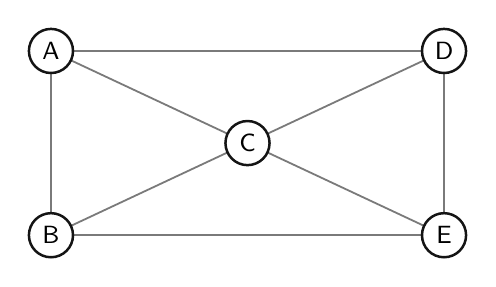
\begin{tikzpicture}[x=0.78cm,y=0.78cm,baseline=(current bounding box.center)]
\coordinate (A) at (0,3);
\coordinate (B) at (0,0);
\coordinate (C) at (3.2,1.5);
\coordinate (D) at (6.4,3);
\coordinate (E) at (6.4,0);
\draw[available] (A) -- (B);
\draw[available] (B) -- (C);
\draw[available] (A) -- (C);
\draw[available] (C) -- (D);
\draw[available] (D) -- (E);
\draw[available] (C) -- (E);
\draw[available] (A) -- (D);
\draw[available] (B) -- (E);
\node[place,minimum size=0.56cm,font=\small] at (A) {A};
\node[place,minimum size=0.56cm,font=\small] at (B) {B};
\node[place,minimum size=0.56cm,font=\small] at (C) {C};
\node[place,minimum size=0.56cm,font=\small] at (D) {D};
\node[place,minimum size=0.56cm,font=\small] at (E) {E};
\end{tikzpicture}
}

\newcommand{\SwapBefore}{%
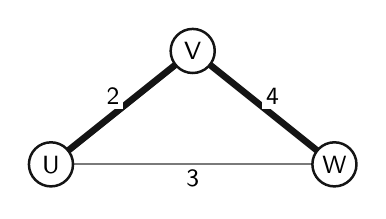
\begin{tikzpicture}[x=0.72cm,y=0.72cm,baseline=(current bounding box.center)]
\coordinate (U) at (0,0);
\coordinate (V) at (2.5,2);
\coordinate (W) at (5,0);
\draw[available] (U) -- (V);
\draw[available] (V) -- (W);
\draw[available] (U) -- (W);
\draw[bought] (U) -- (V);
\draw[bought] (V) -- (W);
\node[price,font=\small] at (1.09383,1.19522) {2};
\node[price,font=\small] at (3.90617,1.19522) {4};
\node[price,font=\small] at (2.50000,-0.25000) {3};
\node[place,minimum size=0.56cm,font=\small] at (U) {U};
\node[place,minimum size=0.56cm,font=\small] at (V) {V};
\node[place,minimum size=0.56cm,font=\small] at (W) {W};
\end{tikzpicture}
}

\newcommand{\SwapMiddle}{%
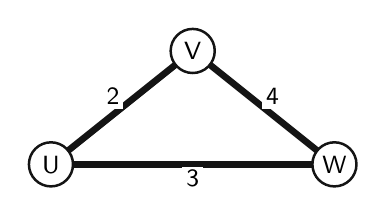
\begin{tikzpicture}[x=0.72cm,y=0.72cm,baseline=(current bounding box.center)]
\coordinate (U) at (0,0);
\coordinate (V) at (2.5,2);
\coordinate (W) at (5,0);
\draw[available] (U) -- (V);
\draw[available] (V) -- (W);
\draw[available] (U) -- (W);
\draw[bought] (U) -- (V);
\draw[bought] (V) -- (W);
\draw[bought] (U) -- (W);
\node[price,font=\small] at (1.09383,1.19522) {2};
\node[price,font=\small] at (3.90617,1.19522) {4};
\node[price,font=\small] at (2.50000,-0.25000) {3};
\node[place,minimum size=0.56cm,font=\small] at (U) {U};
\node[place,minimum size=0.56cm,font=\small] at (V) {V};
\node[place,minimum size=0.56cm,font=\small] at (W) {W};
\end{tikzpicture}
}

\newcommand{\SwapAfter}{%
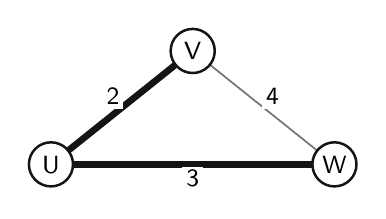
\begin{tikzpicture}[x=0.72cm,y=0.72cm,baseline=(current bounding box.center)]
\coordinate (U) at (0,0);
\coordinate (V) at (2.5,2);
\coordinate (W) at (5,0);
\draw[available] (U) -- (V);
\draw[available] (V) -- (W);
\draw[available] (U) -- (W);
\draw[bought] (U) -- (V);
\draw[bought] (U) -- (W);
\node[price,font=\small] at (1.09383,1.19522) {2};
\node[price,font=\small] at (3.90617,1.19522) {4};
\node[price,font=\small] at (2.50000,-0.25000) {3};
\node[place,minimum size=0.56cm,font=\small] at (U) {U};
\node[place,minimum size=0.56cm,font=\small] at (V) {V};
\node[place,minimum size=0.56cm,font=\small] at (W) {W};
\end{tikzpicture}
}

\newcommand{\SwapFirst}{%
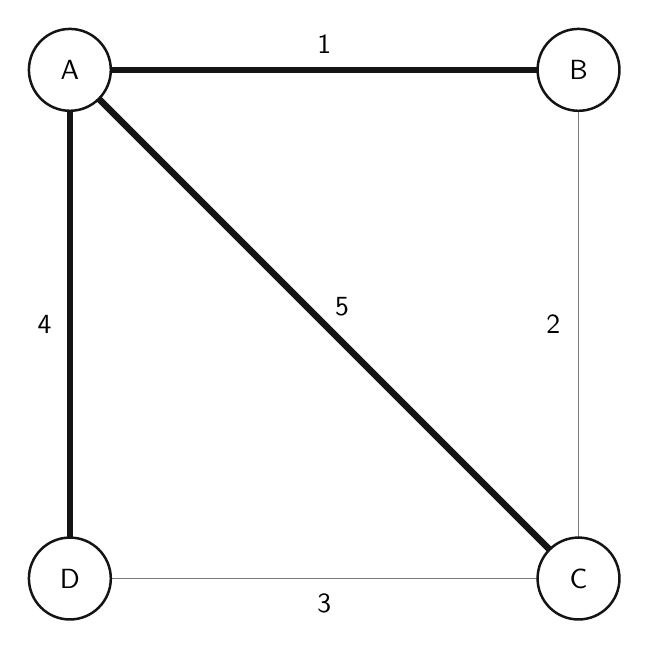
\begin{tikzpicture}[x=1.9cm,y=1.9cm,baseline=(current bounding box.center)]
\coordinate (A) at (0,3.4);
\coordinate (B) at (3.4,3.4);
\coordinate (C) at (3.4,0);
\coordinate (D) at (0,0);
\draw[available] (A) -- (B);
\draw[available] (B) -- (C);
\draw[available] (C) -- (D);
\draw[available] (A) -- (D);
\draw[available] (A) -- (C);
\draw[bought] (A) -- (B);
\draw[bought] (A) -- (D);
\draw[bought] (A) -- (C);
\node[price,font=\normalsize] at (1.70000,3.56842) {1};
\node[price,font=\normalsize] at (3.23158,1.70000) {2};
\node[price,font=\normalsize] at (1.70000,-0.16842) {3};
\node[price,font=\normalsize] at (-0.16842,1.70000) {4};
\node[price,font=\normalsize] at (1.81909,1.81909) {5};
\node[place,minimum size=1.04cm,font=\normalsize] at (A) {A};
\node[place,minimum size=1.04cm,font=\normalsize] at (B) {B};
\node[place,minimum size=1.04cm,font=\normalsize] at (C) {C};
\node[place,minimum size=1.04cm,font=\normalsize] at (D) {D};
\end{tikzpicture}
}

\newcommand{\SwapSecond}{%
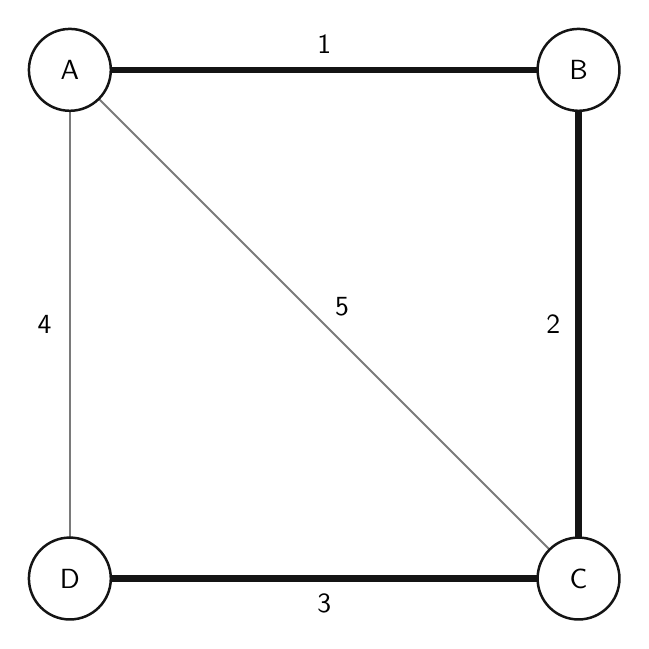
\begin{tikzpicture}[x=1.9cm,y=1.9cm,baseline=(current bounding box.center)]
\coordinate (A) at (0,3.4);
\coordinate (B) at (3.4,3.4);
\coordinate (C) at (3.4,0);
\coordinate (D) at (0,0);
\draw[available] (A) -- (B);
\draw[available] (B) -- (C);
\draw[available] (C) -- (D);
\draw[available] (A) -- (D);
\draw[available] (A) -- (C);
\draw[bought] (A) -- (B);
\draw[bought] (B) -- (C);
\draw[bought] (C) -- (D);
\node[price,font=\normalsize] at (1.70000,3.56842) {1};
\node[price,font=\normalsize] at (3.23158,1.70000) {2};
\node[price,font=\normalsize] at (1.70000,-0.16842) {3};
\node[price,font=\normalsize] at (-0.16842,1.70000) {4};
\node[price,font=\normalsize] at (1.81909,1.81909) {5};
\node[place,minimum size=1.04cm,font=\normalsize] at (A) {A};
\node[place,minimum size=1.04cm,font=\normalsize] at (B) {B};
\node[place,minimum size=1.04cm,font=\normalsize] at (C) {C};
\node[place,minimum size=1.04cm,font=\normalsize] at (D) {D};
\end{tikzpicture}
}

\newcommand{\SixCert}{%
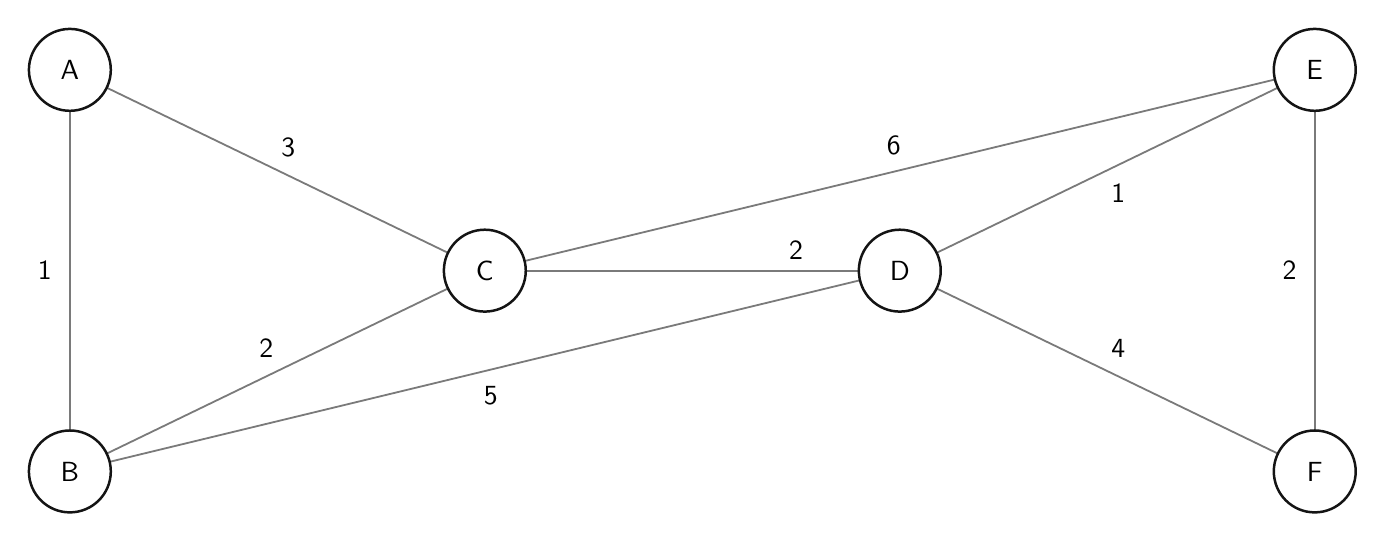
\begin{tikzpicture}[x=1.7cm,y=1.7cm,baseline=(current bounding box.center)]
\coordinate (A) at (0,3);
\coordinate (B) at (0,0);
\coordinate (C) at (3.1,1.5);
\coordinate (D) at (6.2,1.5);
\coordinate (E) at (9.3,3);
\coordinate (F) at (9.3,0);
\draw[available] (A) -- (B);
\draw[available] (B) -- (C);
\draw[available] (A) -- (C);
\draw[available] (C) -- (D);
\draw[available] (D) -- (E);
\draw[available] (E) -- (F);
\draw[available] (D) -- (F);
\draw[available] (B) -- (D);
\draw[available] (C) -- (E);
\node[price,font=\normalsize] at (-0.18824,1.50000) {1};
\node[price,font=\normalsize] at (1.46801,0.91944) {2};
\node[price,font=\normalsize] at (1.63199,2.41944) {3};
\node[price,font=\normalsize] at (5.42500,1.65294) {2};
\node[price,font=\normalsize] at (7.83199,2.08056) {1};
\node[price,font=\normalsize] at (9.11176,1.50000) {2};
\node[price,font=\normalsize] at (7.83199,0.91944) {4};
\node[price,font=\normalsize] at (3.14426,0.56704) {5};
\node[price,font=\normalsize] at (6.15574,2.43296) {6};
\node[place,minimum size=1.04cm,font=\normalsize] at (A) {A};
\node[place,minimum size=1.04cm,font=\normalsize] at (B) {B};
\node[place,minimum size=1.04cm,font=\normalsize] at (C) {C};
\node[place,minimum size=1.04cm,font=\normalsize] at (D) {D};
\node[place,minimum size=1.04cm,font=\normalsize] at (E) {E};
\node[place,minimum size=1.04cm,font=\normalsize] at (F) {F};
\end{tikzpicture}
}

\newcommand{\PriceDesign}{%
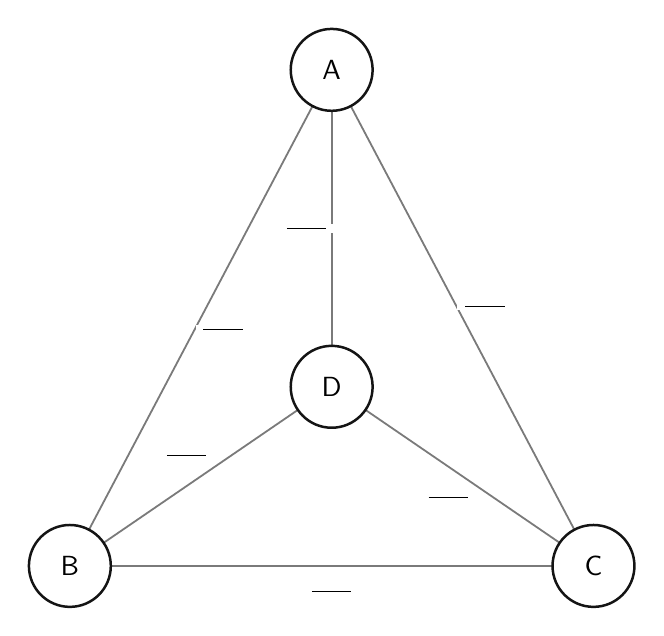
\begin{tikzpicture}[x=1.75cm,y=1.75cm,baseline=(current bounding box.center)]
\coordinate (A) at (1.9,3.6);
\coordinate (B) at (0,0);
\coordinate (C) at (3.8,0);
\coordinate (D) at (1.9,1.3);
\draw[available] (A) -- (B);
\draw[available] (B) -- (C);
\draw[available] (A) -- (C);
\draw[available] (A) -- (D);
\draw[available] (B) -- (D);
\draw[available] (C) -- (D);
\node[price,font=\normalsize] at (1.11172,1.71465) {\makebox[0.6cm]{\rule{0.5cm}{0.35pt}}};
\node[price,font=\normalsize] at (1.90000,-0.18286) {\makebox[0.6cm]{\rule{0.5cm}{0.35pt}}};
\node[price,font=\normalsize] at (3.01172,1.88535) {\makebox[0.6cm]{\rule{0.5cm}{0.35pt}}};
\node[price,font=\normalsize] at (1.71714,2.45000) {\makebox[0.6cm]{\rule{0.5cm}{0.35pt}}};
\node[price,font=\normalsize] at (0.84674,0.80091) {\makebox[0.6cm]{\rule{0.5cm}{0.35pt}}};
\node[price,font=\normalsize] at (2.74674,0.49909) {\makebox[0.6cm]{\rule{0.5cm}{0.35pt}}};
\node[place,minimum size=1.04cm,font=\normalsize] at (A) {A};
\node[place,minimum size=1.04cm,font=\normalsize] at (B) {B};
\node[place,minimum size=1.04cm,font=\normalsize] at (C) {C};
\node[place,minimum size=1.04cm,font=\normalsize] at (D) {D};
\end{tikzpicture}
}

\newcommand{\SixGood}{%
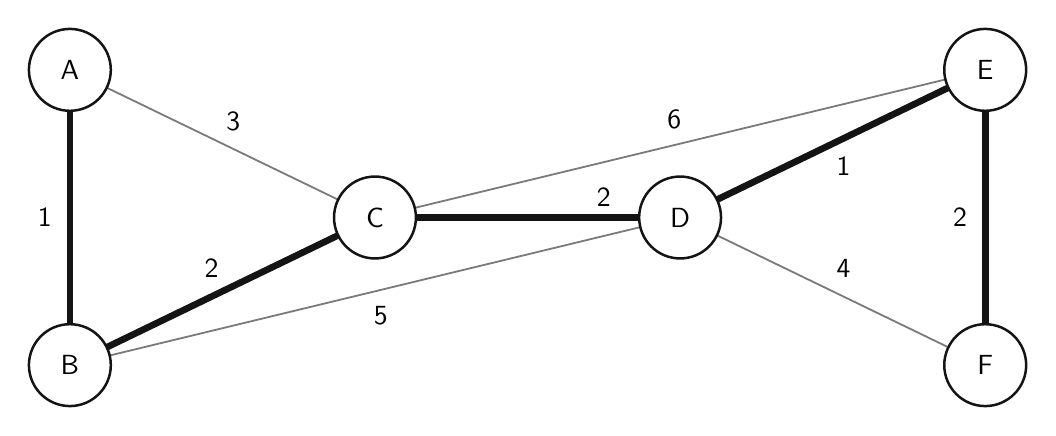
\begin{tikzpicture}[x=1.25cm,y=1.25cm,baseline=(current bounding box.center)]
\coordinate (A) at (0,3);
\coordinate (B) at (0,0);
\coordinate (C) at (3.1,1.5);
\coordinate (D) at (6.2,1.5);
\coordinate (E) at (9.3,3);
\coordinate (F) at (9.3,0);
\draw[available] (A) -- (B);
\draw[available] (B) -- (C);
\draw[available] (A) -- (C);
\draw[available] (C) -- (D);
\draw[available] (D) -- (E);
\draw[available] (E) -- (F);
\draw[available] (D) -- (F);
\draw[available] (B) -- (D);
\draw[available] (C) -- (E);
\draw[bought] (A) -- (B);
\draw[bought] (B) -- (C);
\draw[bought] (C) -- (D);
\draw[bought] (D) -- (E);
\draw[bought] (E) -- (F);
\node[price,font=\normalsize] at (-0.25600,1.50000) {1};
\node[price,font=\normalsize] at (1.43850,0.98044) {2};
\node[price,font=\normalsize] at (1.66150,2.48044) {3};
\node[price,font=\normalsize] at (5.42500,1.70800) {2};
\node[price,font=\normalsize] at (7.86150,2.01956) {1};
\node[price,font=\normalsize] at (9.04400,1.50000) {2};
\node[price,font=\normalsize] at (7.86150,0.98044) {4};
\node[price,font=\normalsize] at (3.16020,0.50118) {5};
\node[price,font=\normalsize] at (6.13980,2.49882) {6};
\node[place,minimum size=1.04cm,font=\normalsize] at (A) {A};
\node[place,minimum size=1.04cm,font=\normalsize] at (B) {B};
\node[place,minimum size=1.04cm,font=\normalsize] at (C) {C};
\node[place,minimum size=1.04cm,font=\normalsize] at (D) {D};
\node[place,minimum size=1.04cm,font=\normalsize] at (E) {E};
\node[place,minimum size=1.04cm,font=\normalsize] at (F) {F};
\end{tikzpicture}
}

\newcommand{\SixBad}{%
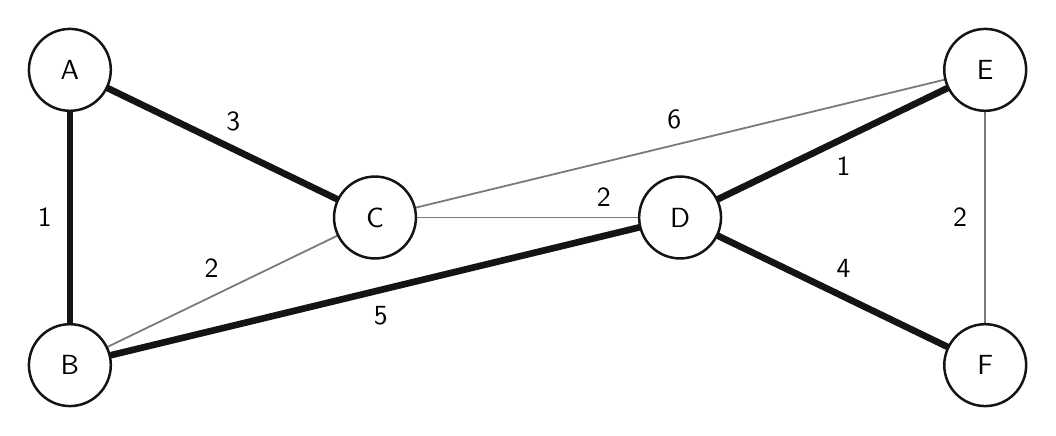
\begin{tikzpicture}[x=1.25cm,y=1.25cm,baseline=(current bounding box.center)]
\coordinate (A) at (0,3);
\coordinate (B) at (0,0);
\coordinate (C) at (3.1,1.5);
\coordinate (D) at (6.2,1.5);
\coordinate (E) at (9.3,3);
\coordinate (F) at (9.3,0);
\draw[available] (A) -- (B);
\draw[available] (B) -- (C);
\draw[available] (A) -- (C);
\draw[available] (C) -- (D);
\draw[available] (D) -- (E);
\draw[available] (E) -- (F);
\draw[available] (D) -- (F);
\draw[available] (B) -- (D);
\draw[available] (C) -- (E);
\draw[bought] (A) -- (B);
\draw[bought] (A) -- (C);
\draw[bought] (D) -- (E);
\draw[bought] (D) -- (F);
\draw[bought] (B) -- (D);
\node[price,font=\normalsize] at (-0.25600,1.50000) {1};
\node[price,font=\normalsize] at (1.43850,0.98044) {2};
\node[price,font=\normalsize] at (1.66150,2.48044) {3};
\node[price,font=\normalsize] at (5.42500,1.70800) {2};
\node[price,font=\normalsize] at (7.86150,2.01956) {1};
\node[price,font=\normalsize] at (9.04400,1.50000) {2};
\node[price,font=\normalsize] at (7.86150,0.98044) {4};
\node[price,font=\normalsize] at (3.16020,0.50118) {5};
\node[price,font=\normalsize] at (6.13980,2.49882) {6};
\node[place,minimum size=1.04cm,font=\normalsize] at (A) {A};
\node[place,minimum size=1.04cm,font=\normalsize] at (B) {B};
\node[place,minimum size=1.04cm,font=\normalsize] at (C) {C};
\node[place,minimum size=1.04cm,font=\normalsize] at (D) {D};
\node[place,minimum size=1.04cm,font=\normalsize] at (E) {E};
\node[place,minimum size=1.04cm,font=\normalsize] at (F) {F};
\end{tikzpicture}
}

\newcommand{\Distinct}{%
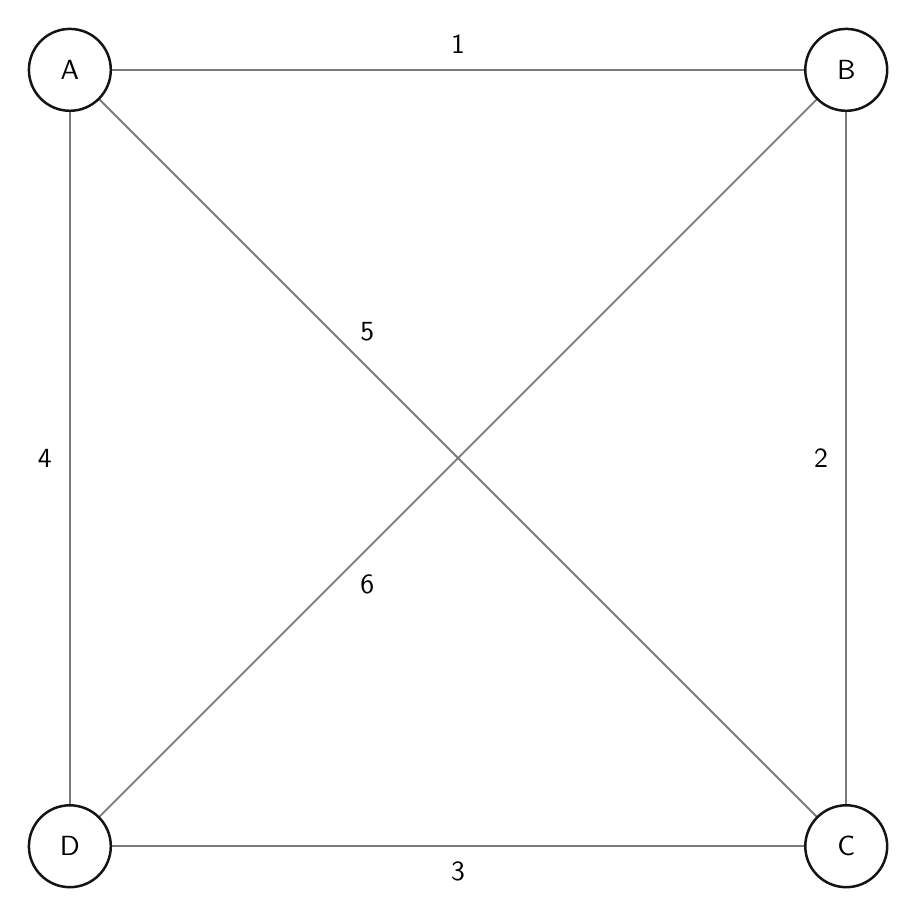
\begin{tikzpicture}[x=2.9cm,y=2.9cm,baseline=(current bounding box.center)]
\coordinate (A) at (0,3.4);
\coordinate (B) at (3.4,3.4);
\coordinate (C) at (3.4,0);
\coordinate (D) at (0,0);
\draw[available] (A) -- (B);
\draw[available] (B) -- (C);
\draw[available] (C) -- (D);
\draw[available] (A) -- (D);
\draw[available] (A) -- (C);
\draw[available] (B) -- (D);
\node[price,font=\normalsize] at (1.70000,3.51034) {1};
\node[price,font=\normalsize] at (3.28966,1.70000) {2};
\node[price,font=\normalsize] at (1.70000,-0.11034) {3};
\node[price,font=\normalsize] at (-0.11034,1.70000) {4};
\node[price,font=\normalsize] at (1.30203,2.25403) {5};
\node[price,font=\normalsize] at (1.30203,1.14597) {6};
\node[place,minimum size=1.04cm,font=\normalsize] at (A) {A};
\node[place,minimum size=1.04cm,font=\normalsize] at (B) {B};
\node[place,minimum size=1.04cm,font=\normalsize] at (C) {C};
\node[place,minimum size=1.04cm,font=\normalsize] at (D) {D};
\end{tikzpicture}
}


Mark whole printed links you buy. Thick links are bought. Pay each link's price once. A price of 2, shown as \pricedots{2}, costs two counters. Return a link to get its counters back. Travel follows bought links and turns only at circled places.

\begin{center}
\begin{tabular}{@{}c@{\hspace{0.28cm}}c@{\hspace{0.28cm}}c@{}}
\small Available links & \small Bought and paid & \small Kept record\\[5pt]
\ExampleAvailable & \ExamplePaid & \ExampleRecord\\[5pt]
 & \small $2+4=6$\quad\coins{6} & \small All 3 places connected\\
\end{tabular}
\end{center}
\vspace{0.12in}

\problem{1}{Connect all three places for the fewest counters on each map.}

\vspace{0.4in}
\begin{center}
\begin{minipage}{0.48\linewidth}\centering\TriangleOne\par\vspace{0.45in}\cost\end{minipage}\hfill
\begin{minipage}{0.48\linewidth}\centering\TriangleTwo\par\vspace{0.45in}\cost\end{minipage}
\end{center}

\newpage

\problem{2}{Find every cheapest purchase that connects all four places.}

\vspace{0.6in}
\begin{center}\FourTies\end{center}
\vspace{0.4in}
\cost
\vspace{0.8in}
\begin{center}
\FourTiesRecord\hfill\FourTiesRecord\hfill\FourTiesRecord
\end{center}
\vspace{0.3in}
\begin{center}
\FourTiesRecord\hspace{1.2in}\FourTiesRecord
\end{center}

\newpage

\problem{3}{Connect all four places for the least total cost. Show why a cheaper purchase cannot work.}

\vspace{0.65in}
\begin{center}\FourTrap\end{center}
\vspace{0.35in}
\cost
\vspace{0.6in}
\begin{center}\FourTrapRecord\hspace{1.2in}\FourTrapRecord\end{center}

\newpage

\problem{4}{Find every cheapest purchase that connects all five places.}

\vspace{0.6in}
\begin{center}\FiveTies\end{center}
\vspace{0.3in}
\cost
\vspace{0.65in}
\begin{center}\FiveTiesRecord\hfill\FiveTiesRecord\hfill\FiveTiesRecord\end{center}
\vspace{0.3in}
\begin{center}\FiveTiesRecord\hspace{1.2in}\FiveTiesRecord\end{center}

\newpage

\renewcommand\Band{Grades 4--5}

\problem{5}{Starting each time from the printed thick purchase, find every cheaper one-link swap: buy one unused link and return one bought link. The result must connect every place.}

\begin{center}
\begin{tabular}{@{}c@{\hspace{0.28cm}}c@{\hspace{0.28cm}}c@{}}
\small Before & \small Buy UW for 3 & \small Return VW for 4\\[4pt]
\SwapBefore & \SwapMiddle & \SwapAfter\\[4pt]
\small Cost 6 & \small Cost 9 & \small Cost 5\\
\end{tabular}
\end{center}
\vspace{0.15in}
\begin{center}
\begin{minipage}{0.48\linewidth}\centering\SwapFirst\par\vspace{0.25in}\swaprows\end{minipage}\hfill
\begin{minipage}{0.48\linewidth}\centering\SwapSecond\par\vspace{0.25in}\swaprows\end{minipage}
\end{center}

\newpage

\problem{6}{Which links must be in every cheapest purchase? Which links are in no cheapest purchase? Give reasons that rule out every competing purchase.}

\vspace{0.7in}
\begin{center}\SixCert\end{center}
\vspace{0.6in}
\begin{minipage}[t]{0.47\linewidth}In every cheapest purchase:\end{minipage}\hfill
\begin{minipage}[t]{0.47\linewidth}In no cheapest purchase:\end{minipage}

\newpage

\problem{7}{Give each link a price of 1, 2, 3 or 4. Make the left map have exactly one cheapest purchase and the right map have at least two. Show why both meet their condition.}

\vspace{0.75in}
\begin{center}
\begin{minipage}{0.48\linewidth}\centering\PriceDesign\end{minipage}\hfill
\begin{minipage}{0.48\linewidth}\centering\PriceDesign\end{minipage}
\end{center}

\newpage

\problem{8}{All link prices are positive. A loop follows bought links back to its start without using a link twice. Can a cheapest purchase contain a loop? For each thick purchase, find a cheaper one-link swap or explain why none exists. Can a connected purchase with no loop cost more than the cheapest one even though no one-link swap makes it cheaper?}

\vspace{0.35in}
\begin{center}\SixGood\end{center}
\vspace{0.25in}
\begin{center}\SixBad\end{center}

\newpage

\problem{9}{Find the cheapest purchase on this map. Can any map with a different positive price on every link have two different cheapest purchases? Explain your answer.}

\vspace{0.4in}
\begin{center}\Distinct\end{center}
\end{document}
